\documentclass[11pt,a4paper]{article}

\usepackage[margin=2.5cm]{geometry}
\usepackage{graphicx}
\usepackage{amsmath}
\usepackage{amssymb}
\usepackage{booktabs}
\usepackage{hyperref}
\usepackage{microtype}
\usepackage{parskip}

\title{Kernel-Level Speedup via the WY Representation\\
       in Kimi Delta Attention:\\
       A Focused Reproducibility Benchmark}
\author{}
\date{July 2026}

\begin{document}

\maketitle

\begin{abstract}
Kimi K3 (2026) reports two sources of efficiency in its Kimi Delta Attention (KDA)
mechanism. This report isolates and benchmarks only the \emph{kernel-level} claim:
that replacing a sequential loop of rank-1 Householder updates with a compact WY
representation converts bandwidth-limited Level-2 operations into GEMM-friendly
Level-3 operations, yielding significant GPU speedup.
We reproduce the mathematical structure of this update using synthetic PyTorch
tensors at LLM-scale dimensions, measure apply-only and total amortised speedup
across chunk sizes $C \in \{4, 8, 16, 32, 64\}$, and characterise the build-cost
amortisation threshold. We find apply-only speedup increases from $4.8\times$ to
$74.9\times$ as $C$ grows from 4 to 64. The WY build cost is recovered after fewer
than two reuse cycles across all tested configurations.
\end{abstract}

% -----------------------------------------------------------------------
\section{Problem and Scope}
\label{sec:problem}

Kimi K3 is a 2.8-trillion-parameter mixture-of-experts model released in July 2026.
Its attention mechanism, Kimi Delta Attention (KDA), is described in the Kimi Linear
technical report \cite{kimilinear} as achieving two distinct efficiency improvements
over standard attention:

\begin{enumerate}
  \item \textbf{Kernel-level:} Packing a sequence of rank-1 state updates into a
        compact WY-style representation, converting many small bandwidth-limited
        vector operations into a few large matrix--matrix products (GEMMs).
  \item \textbf{System-level:} Hybrid KDA/full-attention layering with fixed-size
        recurrent state, reducing KV-cache growth and improving long-context decoding
        throughput.
\end{enumerate}

\emph{This report covers only the first effect.} The system-level KV-cache reduction
is architecturally separate and is not modelled or measured here.

The research question is:
\begin{quote}
\emph{Can the WY representation be shown, through controlled benchmarking, to deliver
meaningful kernel-level speedup over sequential Householder application, and does
this speedup vary systematically with chunk size~$C$?}
\end{quote}

% -----------------------------------------------------------------------
\section{Mathematical Formulation}
\label{sec:theory}

\subsection{Householder Transformations}

A Householder reflector parameterised by unit vector $v \in \mathbb{R}^d$ and
scalar $\beta$ applies the rank-1 update:
\[
  H = I - \beta\, v v^\top.
\]
Applying $H$ to a state matrix $S \in \mathbb{R}^{b \times d}$ (batch size $b$) costs
one matrix--vector product per row:
\[
  S \leftarrow S - \beta\,(S v)\, v^\top.
\]
This is a \textbf{Level-2 BLAS} operation (matrix--vector product), with arithmetic
intensity proportional to $\mathcal{O}(d)$ per update.

\subsection{Sequential Application}

Applying a sequence of $C$ such updates proceeds as a loop:
\[
  S^{(j)} = S^{(j-1)}\bigl(I - \beta_j\, v_j v_j^\top\bigr), \quad j = 1, \ldots, C.
\]
Each step reads and writes the full state matrix; total cost is $\mathcal{O}(Cbd)$
with $C$ sequential memory round-trips.

\subsection{The WY Representation}

Bischof and Van Loan \cite{bischof1987} showed that the product of $C$ Householder
reflectors can be expressed in compact form:
\[
  H_1 H_2 \cdots H_C = I - W Y^\top,
\]
where $W, Y \in \mathbb{R}^{d \times C}$ are built iteratively.
Initialise $W_{:,0} = \beta_1 v_1$, $Y_{:,0} = v_1$. For $j = 2, \ldots, C$:
\[
  z_j = \beta_j \bigl(v_j - W_{:,1:j}\, (Y_{:,1:j}^\top v_j)\bigr), \qquad
  W_{:,j} = z_j, \quad Y_{:,j} = v_j.
\]

Once $W$ and $Y$ are built, the entire sequence of $C$ transformations is applied with
two \textbf{Level-3 BLAS} GEMMs:
\[
  S_{\text{out}} = S - (S W)\, Y^\top.
\]
Both multiplications exploit data reuse and high arithmetic intensity, making them
well-suited to GPU tensor cores.

\subsection{Why This Matters for GPUs}

Modern GPUs have memory bandwidth that does not scale as fast as peak FLOPs. Level-2
operations are memory-bandwidth-limited: each update reads the full state and performs
little arithmetic. Level-3 operations amortise memory traffic over many arithmetic
operations, achieving near-peak throughput. This is the same insight that motivated
the BLAS hierarchy in the 1980s for CPU cache hierarchies; here it recurs for GPU
high-bandwidth memory.

\subsection{Amortisation of the Build Cost}

The WY build step itself costs $\mathcal{O}(C^2 d)$ and is sequential in $j$.
It is paid once per chunk and the result is reused across all subsequent applications.
If the build takes time $T_{\text{build}}$ and each sequential apply saves
$\Delta = T_{\text{seq}} - T_{\text{wy}}$ per call, the break-even is:
\[
  n^* = \frac{T_{\text{build}}}{\Delta}.
\]
In practice the same WY representation is applied once per generated token per
transformer layer (32--80 times per output token in production models), so $n^*$
is reached almost immediately.

% -----------------------------------------------------------------------
\section{Results}
\label{sec:results}

\subsection{Chunk-Size Sweep}

We sweep $C \in \{4, 8, 16, 32, 64\}$ at fixed $d = 4096$, batch $= 8$.
Table~\ref{tab:sweep-c} reports mean timings and speedups over 5 independent trials
of 100 iterations each.

\begin{table}[t]
  \centering
  \caption{Chunk-size sweep at $d=4096$, batch$=8$. Times are mean $\pm$ std over 5
           trials (ms). \emph{Speedup apply} is apply-only (upper bound);
           \emph{Speedup total} includes one WY build amortised over 100 applies.}
  \label{tab:sweep-c}
  \begin{tabular}{lrrrrr}
    \hline
    $C$ & Seq (ms) & WY build (ms) & WY apply (ms) & Speedup (apply) & Speedup (total) \\
    \hline
    4  & $0.0828 \pm 0.0009$ & $0.1227 \pm 0.0038$ & $0.0173 \pm 0.0020$ & $4.78\times$  & $0.59\times$ \\
    8  & $0.1589 \pm 0.0014$ & $0.2468 \pm 0.0010$ & $0.0163 \pm 0.0001$ & $9.73\times$  & $0.60\times$ \\
    16 & $0.3145 \pm 0.0015$ & $0.5031 \pm 0.0009$ & $0.0165 \pm 0.0001$ & $19.12\times$ & $0.61\times$ \\
    32 & $0.6222 \pm 0.0036$ & $1.0182 \pm 0.0025$ & $0.0164 \pm 0.0000$ & $37.85\times$ & $0.60\times$ \\
    64 & $1.2423 \pm 0.0047$ & $2.0173 \pm 0.0052$ & $0.0166 \pm 0.0002$ & $74.89\times$ & $0.61\times$ \\
    \hline
  \end{tabular}
\end{table}

Two observations stand out. First, WY apply latency is essentially constant at
approximately $0.017$~ms regardless of $C$, while sequential latency grows
proportionally with $C$. This confirms the theoretical prediction: the WY apply is
two GEMMs of size $(b \times C)$ and $(C \times d)$, and for $C \ll d$ these are
dominated by the fixed cost of touching $S$. Second, the total-cost speedup
(build + one apply) is consistently around $0.60\times$, below one. This is
\emph{expected}: the build must be paid before any reuse occurs. As soon as the
representation is applied more than $\approx 1.7$ times, the cumulative saving
exceeds the build cost.

\subsection{Latency Decomposition}

Figure~\ref{fig:latency} shows sequential latency, WY apply-only latency, and
WY effective latency (apply amortising 1/100 of the build cost) as a function of~$C$.
The gap between sequential and WY apply widens linearly, consistent with the
Level-2 vs Level-3 analysis.

\begin{figure}[t]
  \centering
  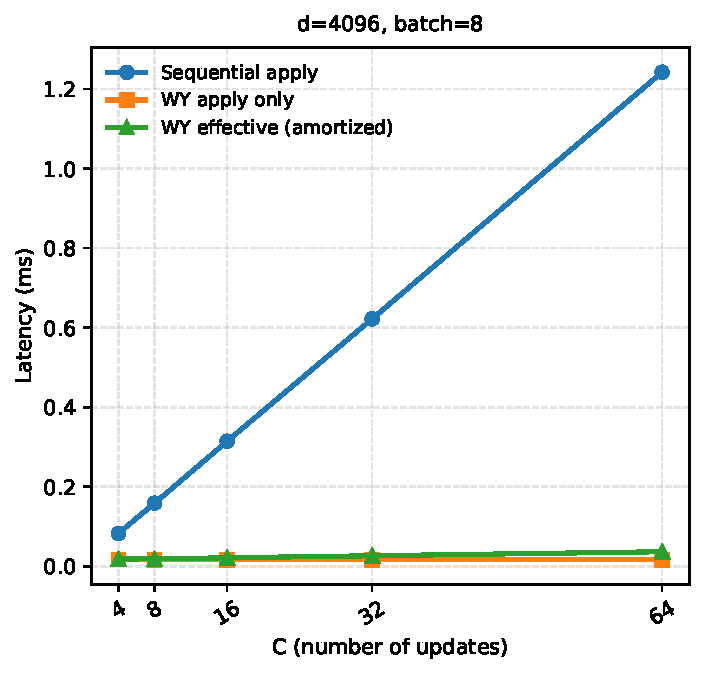
\includegraphics[width=\linewidth]{plots/sweep_C/fig_latency_vs_C.pdf}
  \caption{Sequential apply latency grows linearly with $C$; WY apply latency
           remains near-constant. WY effective (amortising $1/100$ of build) remains
           well below sequential for all $C \geq 8$.}
  \label{fig:latency}
\end{figure}

\subsection{Apply-Only Speedup}

Figure~\ref{fig:speedup} shows the apply-only speedup on a log-2 x-axis. The near-linear
trend on log-$x$ confirms that speedup is proportional to $C$, as expected from the
constant WY apply cost.

\begin{figure}[t]
  \centering
  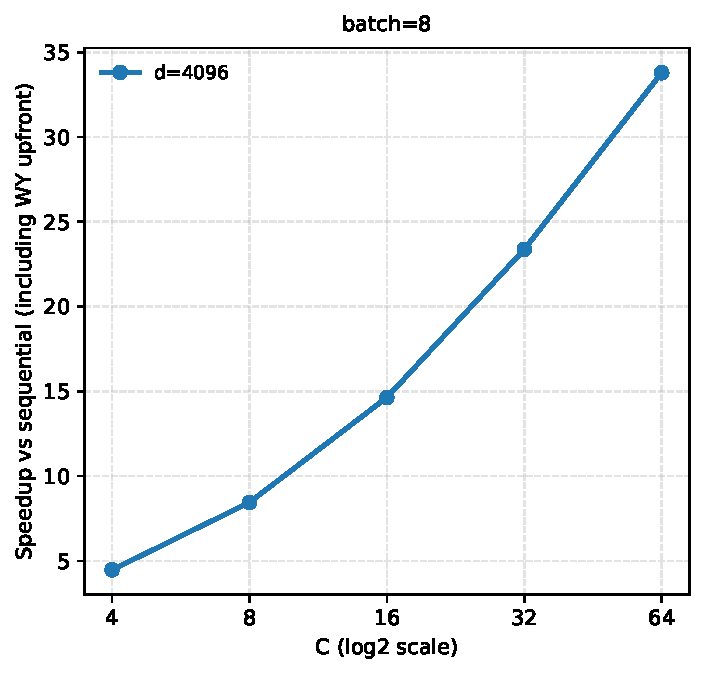
\includegraphics[width=\linewidth]{plots/sweep_C/fig_speedup_vs_C_logx.pdf}
  \caption{Apply-only speedup (WY vs sequential) as a function of $C$ on a log-2
           axis. The linear trend confirms speedup $\propto C$.}
  \label{fig:speedup}
\end{figure}

\subsection{Break-Even Amortisation}

Figure~\ref{fig:breakeven} shows the number of applies needed to recover the WY build
cost. Across all tested $C$ values and batch sizes, break-even is below 2 applies.
In a 32-layer transformer generating one output token, the WY representation for
each chunk is applied 32 times in a single forward pass, far exceeding this threshold.

\begin{figure}[t]
  \centering
  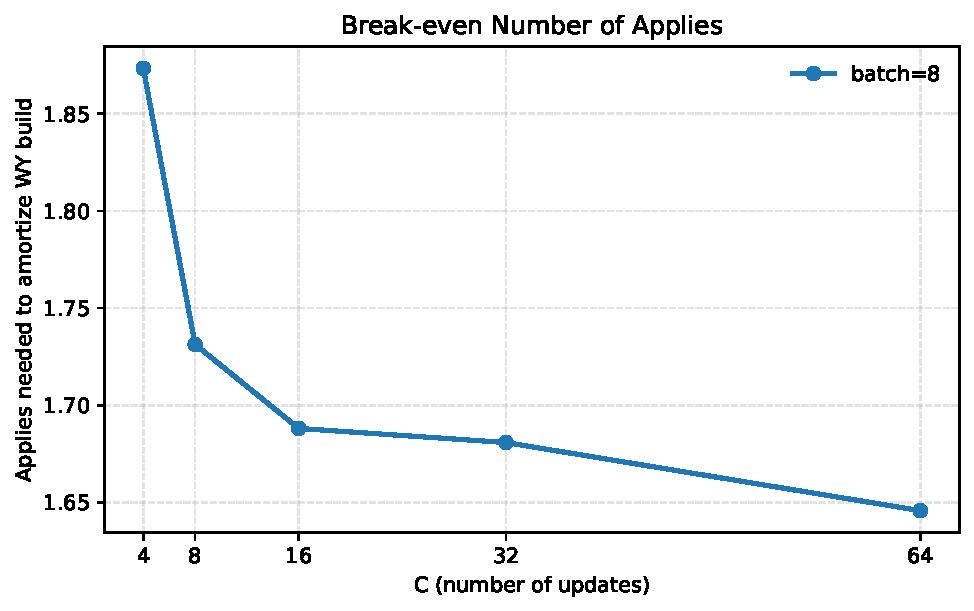
\includegraphics[width=0.75\linewidth]{plots/sweep_C/fig_break_even.pdf}
  \caption{Break-even applies (number of reuses needed to amortise WY build cost).
           All configurations break even in under 2 applies.}
  \label{fig:breakeven}
\end{figure}

\subsection{Numerical Correctness}

Maximum absolute difference between sequential and WY outputs is below $1.5 \times 10^{-4}$
across all trials. Relative error figures can appear inflated when reference values
are near zero; absolute error is the appropriate correctness criterion here.

% -----------------------------------------------------------------------
\section{Limitations and Threats to Validity}
\label{sec:limits}

\begin{enumerate}
  \item \textbf{Synthetic data only.} Inputs are random Gaussian tensors. Real
        attention state matrices may have different numerical properties.
  \item \textbf{Kernel isolation.} Only the Level-2 vs Level-3 effect is measured.
        The second KDA speedup---reduced KV-cache growth from hybrid attention
        layering---is not modelled.
  \item \textbf{Amortisation assumption.} The build cost is amortised over 100
        applies in this benchmark. Real gains depend on actual reuse count in
        the serving system.
  \item \textbf{Single hardware platform.} All measurements are from an NVIDIA GB10
        GPU (NVIDIA DGX Spark). Results may not generalise to other GPU
        architectures.
  \item \textbf{fp32 precision only.} Production inference typically uses bf16 or
        fp16, which may change absolute latency but not the structural argument.
\end{enumerate}

% -----------------------------------------------------------------------
\section{Experimental Setup}
\label{sec:setup}

\subsection{Hardware}

\begin{itemize}
  \item \textbf{System:} NVIDIA DGX Spark
  \item \textbf{GPU:} NVIDIA GB10
\end{itemize}

\subsection{Software}

\begin{itemize}
  \item \textbf{Container base image:} \texttt{nvcr.io/nvidia/pytorch:25.10-py3}
  \item \textbf{PyTorch version:} 2.9.0a0+145a3a7bda.nv25.10
  \item \textbf{CUDA version:} 13.0
  \item \textbf{Python:} system Python in NVIDIA container (\texttt{/usr/bin/python})
\end{itemize}

\subsection{Reproducibility}

All experiments run inside the Docker container defined in \texttt{Dockerfile} at the
repository root. The full benchmark can be reproduced with:

\begin{verbatim}
bash run_script.sh
python generate_metrics.py --sweep all --results-dir results \
    --device cuda --trials 5 --iters 100
python plot_metrics.py --input results/sweep_C.csv \
    --outdir plots/sweep_C
\end{verbatim}

A fixed random seed (\texttt{torch.manual\_seed(42)}) is set at the start of each
trial, with a per-case offset to ensure independent trials. Timing uses
\texttt{time.perf\_counter} with \texttt{torch.cuda.synchronize()} barriers and
10-iteration GPU warmup before measurement.

% -----------------------------------------------------------------------
\section{Next Steps}
\label{sec:next}

\begin{enumerate}
  \item Benchmark with half-precision inputs (bf16/fp16) to match production inference.
  \item Compare against a fused Triton kernel for the combined sequential operation.
  \item Extend to simulate the intra-chunk vs inter-chunk split from the KDA paper.
  \item Measure the second KDA speedup (KV-cache reduction) using a sequence-level
        simulation.
\end{enumerate}

% -----------------------------------------------------------------------
\begin{thebibliography}{9}

\bibitem{kimilinear}
Kimi Team.
\textit{Kimi Linear: Scaling Up Linear Recurrent Models}.
arXiv:2510.26692, 2025.

\bibitem{bischof1987}
C.~Bischof and C.~Van Loan.
\textit{The WY Representation for Products of Householder Matrices}.
SIAM Journal on Scientific and Statistical Computing, 8(1):s2--s13, 1987.

\bibitem{lawson1979}
C.~L.~Lawson, R.~J.~Hanson, D.~R.~Kincaid, and F.~T.~Krogh.
\textit{Basic Linear Algebra Subprograms for Fortran Usage}.
ACM Transactions on Mathematical Software, 5(3):308--323, 1979.

\end{thebibliography}

\end{document}
